\documentclass[12pt]{article}

\usepackage{hyperref}
\usepackage[width=6in,height=8in]{geometry}
\usepackage{guitardiagrams}
\usepackage{graphicx}
\usepackage{float}

\usepackage{pdfpages}


\usepackage{amsthm}
\theoremstyle{definition}
\newtheorem{exercise}{Exercise}


\title{Strumming On A Grid}
\author{Addison Ballif}
\date{\today}

\begin{document}

\maketitle

Much of the time the thing that determines whether a note is picked up or picked down is determined by what is called a grid.
A grid determines how notes are picked based on which part of the measure they fall on. 
Grids also determine what kinds of strumming patterns we can make. 

We will look at a couple of these. 

\section{Eighth Note Grid}
The eighth note grid is the one to use when your fastest note is an eighth note. 
It puts the down strokes on the beat and the up strokes on the off-beats. 
The eighth note grid is shown below, where the down stroke is notated using the open square shaped symbol, and the up stroke is notated with the V shaped symbol. 

\begin{center}
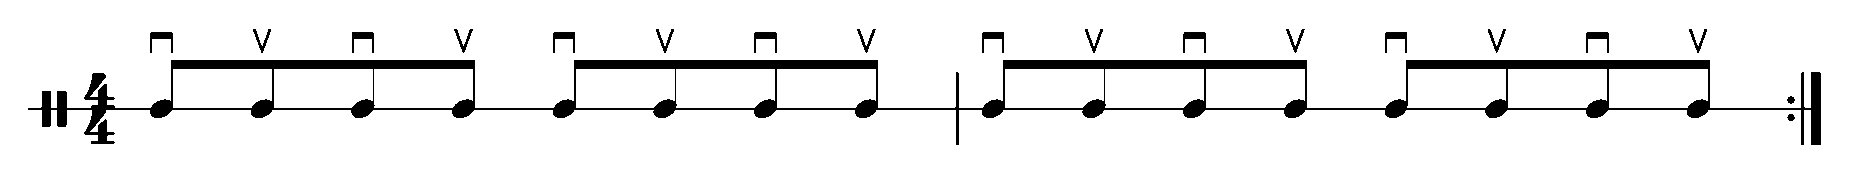
\includegraphics[width=\linewidth]{eighthnotegrid.png}
\end{center}

If we want to play a particular strum pattern, we use this grid and simply remove the notes that we don't want. 
When we remove notes, we still move our hand or arm, but simply miss the string. 
This gives our arm or hand a constant alternating motion that is not interrupted by the rhythm being played. 

\newpage

\begin{exercise}
Try playing the following strum patterns using the eighth note grid by removing the notes not needed. 
First play them by strumming the strings while muting them with your left hand. 
Then practice them plucking a single note. 
Practice that with a metronome set to 80 BPM. When that is comfortable move to 100 BPM, then 120 BPM. 
\end{exercise}

\begin{center}
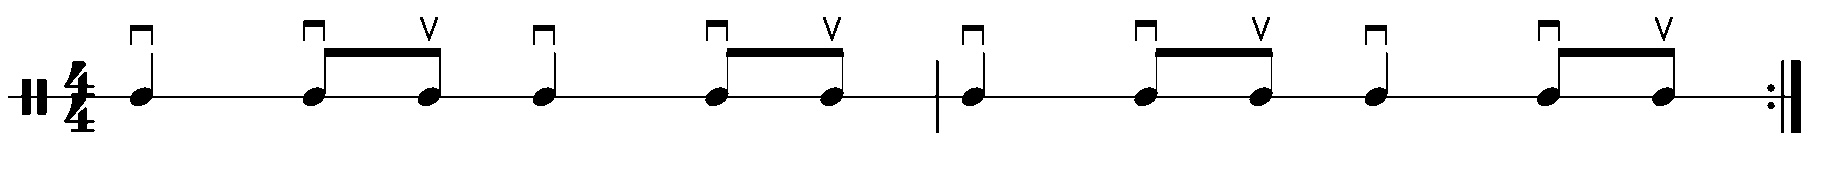
\includegraphics[width=\linewidth]{strum01.png}
\end{center}

\begin{center}
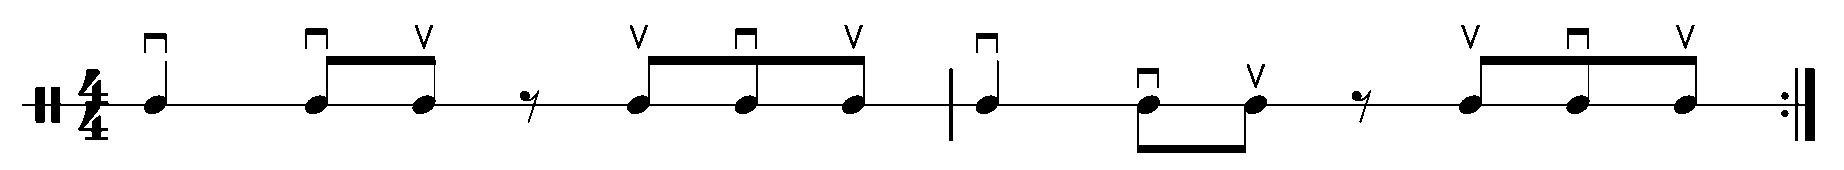
\includegraphics[width=\linewidth]{strum02.png}
\end{center}

\begin{center}
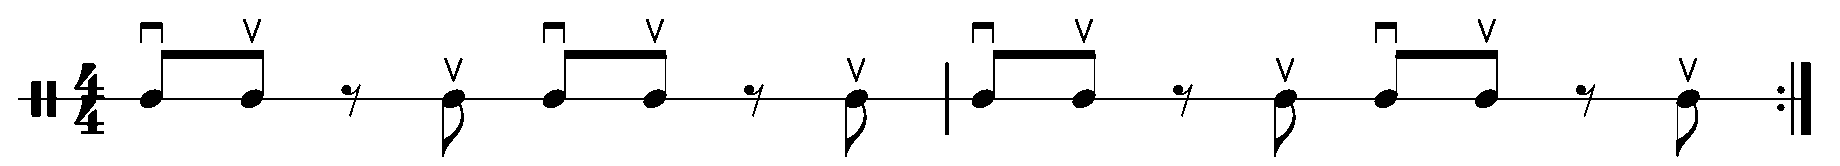
\includegraphics[width=\linewidth]{strum03.png}
\end{center}



\end{document}
